\chapter{Elicitazione dei requisiti}
L'obiettivo comprendere il dominio in cui stiamo lavorando e 
raccogliere e capire i requisiti del software che dovrà essere
implementato. 
\section{Acquisizione della conoscenza}

L'acquisizione della conoscenza è una fase cruciale nel processo di
ingegneria dei requisiti e include diverse attività importanti.

In primo luogo, è essenziale studiare il sistema attuale, noto come sistema
\textit{as-is}. Questo studio comprende la comprensione dell'organizzazione
aziendale (\textit{struttura, dipendenze, obiettivi strategici, politiche, flussi di
lavoro e procedure operative}) e del dominio applicativo (\textit{concetti, obiettivi,
compiti, vincoli e regolamenti}). Inoltre, è necessario analizzare i problemi
esistenti nel sistema attuale, identificandone sintomi, cause e conseguenze.

Un'altra attività chiave è l'analisi delle opportunità tecnologiche e delle
nuove condizioni di mercato, per valutare le possibilità offerte dalle nuove
tecnologie e comprendere come i cambiamenti nelle condizioni di mercato possano
influenzare il sistema.

Identificare gli stakeholder del sistema è fondamentale. Gli stakeholder sono
tutte le parti interessate che hanno un'influenza o sono influenzate dal sistema.
Comprendere le loro esigenze e aspettative è vitale per il successo del progetto.

L'identificazione degli obiettivi di miglioramento per il sistema futuro, noto
come sistema \textit{to-be}, è un'altra attività importante. Questo include
l'analisi dei vincoli organizzativi e tecnici, l'esplorazione di opzioni
alternative, la definizione delle responsabilità e lo sviluppo di scenari
ipotetici di interazione tra software e ambiente. Infine, è cruciale stabilire
i requisiti specifici per il software e fare assunzioni sull'ambiente operativo.

Queste attività forniscono una base solida per il processo di ingegneria
dei requisiti, assicurando che il sistema sviluppato soddisfi le esigenze
degli stakeholder e funzioni efficacemente nel suo ambiente operativo.

Ci sono sostanzialmente due macro-approcci per l'acquisizione della conoscenza:
\begin{itemize}
    \item \textbf{Artefact-driven}: Questo approccio si basa sull'analisi
    di documenti, modelli e altri artefatti esistenti per comprendere il
    sistema attuale e identificare i requisiti del sistema futuro. È
    utile quando il sistema attuale è ben documentato e i requisiti
    del sistema futuro sono chiari.
    \item \textbf{Stakeholder-driven}: Questo approccio si basa sull'interazione
    diretta con gli stakeholder per comprendere le loro esigenze e aspettative
    e identificare i requisiti del sistema futuro. È utile quando il sistema
    attuale è poco documentato o i requisiti del sistema futuro sono incerti.
\end{itemize}
\subsection{Analisi degli stakeholder}

\begin{tcolorbox}[colback=blue!5!white,colframe=blue!75!black]
    Gli stakeholder sono tutte le parti interessate che hanno un'influenza o sono
    influenzate dal sistema.
\end{tcolorbox}

La cooperazione degli stakeholder è essenziale per il
successo dell'ingegneria dei requisiti. Il processo di elicitazione de
 requisiti può essere visto come un apprendimento cooperativo, dove la
 collaborazione tra tutte le parti coinvolte porta a una migliore comprensione
 dei requisiti del sistema.

Per garantire una copertura adeguata e comprensiva del mondo dei problemi,
è necessario selezionare un campione rappresentativo degli stakeholder.
Questa selezione deve essere dinamica, adattandosi man mano che si acquisiscono
nuove conoscenze.

La selezione degli stakeholder si basa su diversi criteri, tra cui:

\begin{itemize}
    \item La posizione rilevante nell'organizzazione.
    \item Il ruolo nella presa di decisioni e nel raggiungimento degli accordi.
    \item Il tipo di conoscenza contribuita e il livello di competenza nel dominio.
    \item L'esposizione ai problemi percepiti.
    \item Gli interessi personali e i potenziali conflitti.
    \item L'influenza nell'accettazione del sistema.
\end{itemize}

Selezionare gli stakeholder giusti è cruciale per assicurare che tutte le
prospettive rilevanti siano considerate e che il sistema finale soddisfi le
esigenze di tutti gli interessati.

\subsection{Difficoltà nell'acquisizione della conoscenza dagli stakeholder}

L'acquisizione della conoscenza dagli stakeholder presenta diverse difficoltà,
tra cui fonti di informazione distribuite, punti di vista conflittuali e
difficoltà di accesso alle persone chiave e ai dati. Gli stakeholder possono
avere background, terminologie e culture differenti, e la conoscenza tacita o
le esigenze nascoste possono complicare ulteriormente il processo. Inoltre,
i dettagli irrilevanti, la politica interna, la competizione e la resistenza
al cambiamento possono influire negativamente.

Il turnover del personale e i cambiamenti organizzativi e delle priorità
possono creare ulteriori sfide. 

Per superare queste difficoltà, sono essenziali abilità di comunicazione,
costruzione di relazioni di fiducia e riformulazione continua della conoscenza
attraverso riunioni di revisione.
\section{Tecniche di Elicitazione guidate dagli Artefatti}
\subsection{Studio del background}

Il processo di acquisizione della conoscenza inizia con la raccolta, la
lettura e la sintesi dei documenti pertinenti. Questi documenti riguardano:

\begin{itemize}
    \item \textbf{L'organizzazione}: include organigrammi, piani aziendali, 
    rapporti finanziari, verbali di riunioni, ecc.
    \item \textbf{Il dominio}: comprende libri, indagini, articoli, regolamenti
    e rapporti su sistemi simili nello stesso dominio.
    \item \textbf{Il sistema attuale (as-is)}: include flussi di lavoro
    documentati, procedure, regole aziendali, documenti scambiati, rapporti
    di difetti/reclami, richieste di modifica, ecc.
\end{itemize}

Questo studio fornisce le basi necessarie per prepararsi prima di incontrare
gli stakeholder e rappresenta un prerequisito per altre tecniche. Tuttavia,
un problema comune è la gestione di una grande quantità di documentazione,
dettagli irrilevanti e informazioni obsolete. La soluzione è utilizzare la
meta-conoscenza per selezionare le informazioni rilevanti, sapendo cosa è
necessario conoscere e cosa non lo è.

\subsection{Raccolta dei dati}

La raccolta dei dati è un'attività importante che si concentra sulla raccolta
di fatti e cifre non documentati. Questi dati possono includere informazioni
di marketing, statistiche di utilizzo, dati sulle prestazioni e costi. La
raccolta può avvenire tramite esperimenti progettati o tramite la selezione
di set di dati rappresentativi da fonti disponibili, utilizzando tecniche di
campionamento statistico.

Questa attività può integrare lo studio del background, fornendo ulteriori
informazioni utili per l'elicitazione dei requisiti non funzionali relativi
a prestazioni, usabilità e costi.

Tuttavia, ci sono alcune difficoltà nella raccolta dei dati. Ottenere dati
affidabili può richiedere tempo e i dati devono essere interpretati
correttamente per essere utili.
\subsection{Questionari}

L'utilizzo dei questionari è un metodo efficace per raccogliere informazioni
dagli stakeholder in modo rapido, economico e a distanza. I questionari
consistono in una lista di domande inviate agli stakeholder selezionati,
ognuna con una lista di possibili risposte. Possono includere:

\begin{itemize}
    \item \textit{Domande a scelta multipla}: dove si seleziona una risposta
    da una lista di opzioni.
    \item \textit{Domande con pesatura}: dove si chiede di attribuire un peso
    a una lista di affermazioni, qualitativamente (ad esempio, ``alto'' o ``basso'')
    o quantitativamente (percentuali), per esprimere l'importanza percepita,
    le preferenze, i rischi, ecc.
\end{itemize}

I questionari sono utili per ottenere rapidamente informazioni soggettive da
molte persone e possono essere d'aiuto nella preparazione di interviste più
focalizzate.

Tuttavia, i questionari devono essere preparati con attenzione per evitare
bias multipli (\textit{dei destinatari, dei rispondenti, delle domande, delle risposte})
e informazioni inaffidabili dovute a fraintendimenti o risposte incoerenti.

Ecco alcune linee guida per la progettazione e la validazione dei questionari:

\begin{itemize}
    \item Selezionare un campione rappresentativo e statisticamente significativo
    di persone, fornendo motivazioni per rispondere.
    \item Verificare la copertura delle domande e delle possibili risposte.
    \item Assicurarsi che le domande e le formulazioni siano imparziali e non
    ambigue.
    \item Aggiungere domande ridondanti implicitamente per rilevare risposte
    incoerenti.
    \item Far controllare il questionario da una terza parte.
\end{itemize}

\begin{tcolorbox}[colback=green!5!white,colframe=green!75!black, title=Pro dei questionari]
    \begin{itemize}
        \item Raccolta rapida di informazioni
        \item Economici e facili da distribuire
        \item Utili per preparare interviste focalizzate
    \end{itemize}
\end{tcolorbox}

\begin{tcolorbox}[colback=red!5!white,colframe=red!75!black, title=Contro dei questionari]
    \begin{itemize}
        \item Possibili bias dei destinatari e rispondenti
        \item Rischio di fraintendimenti nelle domande e risposte
        \item Difficoltà nell'assicurare risposte coerenti
    \end{itemize}
\end{tcolorbox}

\subsection{Card sorting e repertory grids}

L'obiettivo del card sorting e delle repertory grids è acquisire ulteriori
informazioni sui concetti già elicitati. Nel card sorting, si chiede agli
stakeholder di dividere un set di carte, ognuna rappresentante un concetto,
in sottogruppi basati sui loro criteri. Per ogni sottogruppo, si indaga sulle 
proprietà condivise utilizzate per la classificazione. Questo processo è 
iterativo e può essere ripetuto per nuovi raggruppamenti e proprietà.

Ad esempio, nel contesto di un sistema di pianificazione delle riunioni, 
le carte ``Riunione'' e ``Partecipante'' potrebbero essere raggruppate insieme, 
suggerendo che \textit{i partecipanti devono essere invitati alla riunione}. Nella 
successiva iterazione, lo stesso raggruppamento potrebbe indicare che
\textit{i vincoli dei partecipanti per la riunione devono essere conosciuti}.

Nel repertory grid, si chiede agli stakeholder di caratterizzare un concetto
attraverso attributi e intervalli di valori, formando una griglia
concetto-attributo. Ad esempio, per il concetto di ``Riunione'', gli attributi
potrebbero essere \textit{Data} (Lun-Ven) e \textit{Luogo} (Europa).

Il conceptual laddering, invece, richiede agli stakeholder di classificare
i concetti target lungo collegamenti di classe-sottoclasse, come ad esempio
\texttt{RiunioneRegolare} e \texttt{RiunioneOccasionale} come sottoclassi
di \texttt{Riunione}.

Questi metodi sono semplici, economici e facili da usare per l'elicitazione
rapida di informazioni mancanti, ma i risultati possono essere soggettivi,
irrilevanti o inaccurati.

\begin{tcolorbox}[colback=green!5!white,colframe=green!75!black, title=Pro del card sorting e repertory grids]
    \begin{itemize}
        \item Semplici ed economici
        \item Facili da usare
        \item Rapida elicitazione di informazioni
    \end{itemize}
\end{tcolorbox}

\begin{tcolorbox}[colback=red!5!white,colframe=red!75!black, title=Contro del card sorting e repertory grids]
    \begin{itemize}
        \item Risultati possono essere soggettivi
        \item Possibilità di informazioni irrilevanti
        \item Possibili inaccuratezze nei risultati
    \end{itemize}
\end{tcolorbox}

\subsection{Scenari e storyboard}

Gli scenari e gli storyboard aiutano ad acquisire o validare informazioni
attraverso esempi concreti e narrazioni. Gli scenari illustrano sequenze
tipiche di interazione tra i componenti del sistema per raggiungere un
obiettivo implicito, utilizzati sia per spiegare il sistema attuale
(\textit{as-is}) che per esplorare il sistema futuro (\textit{to-be}).

Gli storyboard raccontano una storia attraverso una sequenza di istantanee,
che possono essere frasi, schizzi, diapositive o immagini, e possono includere
annotazioni che spiegano chi sono i partecipanti, cosa accade loro, perché
accade e cosa succede in caso di eventi alternativi.

Le storyboard possono essere inoltre \textit{passive} o \textit{attive}. Le 
passive se raccontiamo la nostra idea per ricevere un feedback, quindi sono 
adatte per la validazione dei requisiti. Le attive vengono elaborate o 
completate dagli stakeholder, quindi sono adatte per l'elicitazione dei
requisiti.

Gli scenari possono essere:

\begin{itemize}
    \item \textit{Scenario positivo}: un comportamento che il sistema dovrebbe
    coprire.
    \item \textit{Scenario negativo}: un comportamento che il sistema dovrebbe
    escludere.
    \item \textit{Scenario normale}: tutto procede come previsto.
    \item \textit{Scenario anomalo}: una sequenza di interazione desiderata in
    situazioni di eccezione.
\end{itemize}

\begin{tcolorbox}[colback=green!5!white,colframe=green!75!black, title=Pro degli
    scenari]
    \begin{itemize}
        \item Esempi concreti e contro-esempi
        \item Stile narrativo (\textit{recepibili da tutti})
        \item Producono sequenze di animazione, possono essere tradotti in test di accettazione
    \end{itemize}
\end{tcolorbox}

\begin{tcolorbox}[colback=red!5!white,colframe=red!75!black, title=Contro degli
    scenari]
    \begin{itemize}
        \item Inerentemente parziali (\textit{problema di copertura del test})
        \item Esplosione combinatoria (\textit{cf. tracce di programma})
        \item Sovraspecificazione potenziale: sequenze non necessarie, decisioni 
        premature.
        \item Possono contenere dettagli irrilevanti, granularità incompatibili
        tra diversi stakeholder
        \item Mantengono i requisiti impliciti
    \end{itemize}
\end{tcolorbox}

Nonostante ciò, sono preziosi come veicoli iniziali per l'elicitazione dei
requisiti.

\subsection{Prototipi e mock-up}

L'obiettivo dei prototipi e dei mock-up è verificare l'adeguatezza dei requisiti
attraverso il feedback diretto degli utenti, mostrando uno schizzo ridotto del
software futuro in azione. Questo metodo si concentra su requisiti poco chiari
e difficili da formulare per elicitare ulteriori dettagli.

Un prototipo è un'implementazione rapida di alcuni aspetti del sistema:
\begin{itemize}
    \item \textit{Prototipo funzionale}: si focalizza su requisiti funzionali
    specifici, come l'avvio di una riunione o la raccolta dei vincoli dei
    partecipanti.
    \item \textit{Prototipo dell'interfaccia utente}: si concentra sulla
    usabilità, mostrando moduli di input-output e pattern di dialogo.
\end{itemize}

I prototipi possono essere implementati rapidamente utilizzando linguaggi
di programmazione di alto livello, linguaggi di specifica eseguibile, e
servizi generici.

\textit{Prototipazione dei requisiti} include due approcci principali:
\begin{itemize}
    \item \textit{Mock-up}: il prototipo viene scartato una volta che ha
    soddisfatto il suo scopo di chiarire e validare i requisiti.
    \item \textit{Prototipo evolutivo}: il prototipo viene trasformato
    e perfezionato fino a diventare parte del prodotto finale.
\end{itemize}

\begin{tcolorbox}[colback=green!5!white,colframe=green!75!black, title=Pro
    dei prototipi e mock-up]
    \begin{itemize}
        \item Forniscono un'idea concreta di come sarà il software
        \item Chiariscono i requisiti, elicitano quelli nascosti, migliorano
        l'adeguatezza, e aiutano a comprendere le implicazioni
        \item Utili anche per la formazione degli utenti e come stub per test
        di integrazione
    \end{itemize}
\end{tcolorbox}

\begin{tcolorbox}[colback=red!5!white,colframe=red!75!black, title=Contro
    dei prototipi e mock-up]
    \begin{itemize}
        \item Non coprono tutti gli aspetti del sistema
        \item Possono mancare funzionalità importanti
        \item Ignorano requisiti non funzionali rilevanti
        (\textit{prestazioni, costi, ecc.})
        \item Possono creare aspettative troppo alte e fuorvianti
        \item Codice ``quick-and-dirty" difficile da riutilizzare per lo sviluppo
        del software
        \item Potenziali incongruenze tra codice modificato e requisiti documentati
    \end{itemize}
\end{tcolorbox}
\subsection{Riutilizzo della Conoscenza}

L'obiettivo del riutilizzo della conoscenza è accelerare
l'elicitazione attraverso il riutilizzo delle esperienze con sistemi simili
o domini analoghi.
Questo include la conoscenza di organizzazioni simili, domini, e mondi problematici,
come requisiti, assunzioni, proprietà del dominio, ecc.

La trasposizione di conoscenze da un contesto all'altro avviene mediante tre passaggi:
\begin{itemize}
    \item \textit{Istanziazione}: quello viene fatto è un esempio di ciò che è 
    stato visto.
    \item \textit{Specializzazione}: concretizzazione dell'astrazione 
    dell'istanziazione.
    \item \textit{Riformulazione}: adattamento del concetto alla nuova situazione.
\end{itemize}
\subsubsection{Riutilizzo della conoscenza indipendente dal dominio: tassonomie}
Spesso è utile adottare una tassonomia in modo da utilizzare esperienza già maturata.
Tale tassonomia può essere creata mediante l'esperienza in vari contesti in modo 
da facilitare il riutilizzo della conoscenza e la velocità nella raccolta dei requisiti.
\subsubsection{Riutilizzo della conoscenza dipendente dal dominio: meta-modelli}
Come informazioni di riuso è possibile riutilizzare dei meta-modelli elaborati, un 
meta-modello è un modello di modelli, cioè un modello che descrive come costruire
altri modelli. Questo permette di avere una visione più astratta e di poter
riutilizzare la conoscenza in modo più efficace.
\begin{figure}[H]
    \centering
    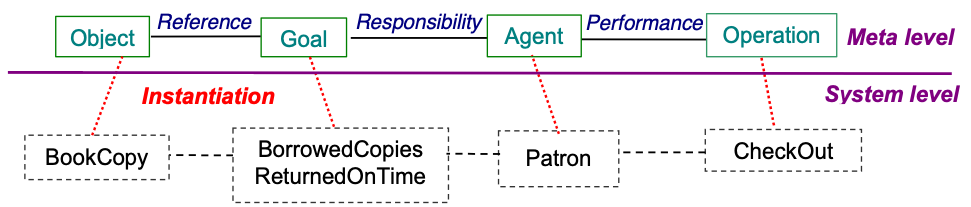
\includegraphics[scale=0.4]{img/metamodel.png}
    \caption{Esempio di meta-modello}
\end{figure}
\subsubsection{Riutilizzo della conoscenza specifica del dominio}
È possibile inoltre utilizzare informazione specifica del dominio astratto, 
sempre avendo come riferimento il modello, sappiamo che ci sono delle risorse che
hanno vincoli di utilizzo limitato, quindi possiamo utilizzare queste informazioni
per capire come si comporterà il sistema.
\[
\textit{Un \textbf{utente} non deve \textbf{usare} più di X \textbf{risorse}
contemporaneamente}
\] 
\[
\textit{Un \textbf{patron} non deve \textbf{prendere in prestito} più di X
\textbf{copie di libri} contemporaneamente}
\]
Questa conoscenza piò essere personalizzata in diversi modi:
\begin{itemize}
    \item Lo stesso dominio astratto può avere molte specializzazioni concrete.
    \item Lo stesso dominio con vincoli diversi può avere molte specializzazioni astratte.
    \item Di fatto posso riusare molteplici strutture.
\end{itemize}
\begin{tcolorbox}[colback=green!5!white,colframe=green!75!black, title=Pro del riutilizzo della conoscenza]
    \begin{itemize}
        \item Analisti esperti riutilizzano la conoscenza acquisita naturalmente
        \item Guida molto nell'elicitazione dei requisiti.
        \item Si eredita la struttura e uindi anche la qualità del dominio che stiamo 
        utilizzando.
        \item È efficace nel completamento del documento dei requisiti.
    \end{itemize}
\end{tcolorbox}
\begin{tcolorbox}[colback=red!5!white,colframe=red!75!black, title=Contro del riutilizzo della conoscenza]
    \begin{itemize}
        \item Possiamo utilizzare la conoscenza astratta solo quando i domini sono
        simili.
        \item Definire i domini astratti è difficile.
        \item C'è effort aggiuntivo per la creazione di meta-modelli.
        \item Quando il dominio si avvicina molto richiede un adattamento complesso.
    \end{itemize}
\end{tcolorbox}
\section{Tecniche di Elicitazione guidate dagli Stakeholder}
\subsection{Interviste}

L'intervista è uno strumento fondamentale per l'acquisizione di conoscenza, permettendo
di catturare informazioni direttamente dai portatori di conoscenza come esperti di
dominio, manager e utenti finali. L'obiettivo principale dell'intervista è di elicitare
informazioni che non emergerebbero tramite altri metodi, focalizzandosi sulle percezioni
personali e sulle esperienze dei partecipanti.

\begin{itemize}
    \item \textit{Preparazione dell'intervista}: L'intervistatore deve selezionare
    accuratamente i partecipanti in base alla loro esperienza e al ruolo ricoperto,
    preparare in anticipo le domande e organizzare incontri che facilitino una
    comunicazione aperta e onesta.
    \item \textit{Conduzione dell'intervista}: La fase di intervista può includere
    sia parti strutturate, con domande specifiche, sia parti non strutturate, che
    permettono di esplorare nuove aree attraverso una discussione libera.
\end{itemize}

\textit{Efficacia dell'intervista} dipende dalla capacità dell'intervistatore di
gestire la conversazione, mantenendo il controllo dell'intervista pur permettendo
all'intervistato di esprimersi liberamente. Le interviste possono svelare dettagli
critici sul funzionamento interno del sistema che non sono immediatamente evidenti
attraverso l'analisi documentale o osservazione diretta.

\begin{tcolorbox}[colback=green!5!white,colframe=green!75!black, title=Pro delle interviste]
    \begin{itemize}
        \item Forniscono intuizioni profonde e dirette dal campo
        \item Permettono la scoperta di requisiti impliciti o non documentati
        \item Aiutano a comprendere meglio le necessità e le preoccupazioni degli utenti
    \end{itemize}
\end{tcolorbox}

\begin{tcolorbox}[colback=red!5!white,colframe=red!75!black, title=Contro delle interviste]
    \begin{itemize}
        \item Possono essere influenzate dalla soggettività degli intervistati
        \item Richiedono tempo e possono essere costose in termini di organizzazione e
        analisi
        \item Le informazioni raccolte possono essere inconsistenti tra diversi intervistati
    \end{itemize}
\end{tcolorbox}

L'approccio misto, combinando elementi di interviste strutturate e non strutturate, è
spesso il più efficace, permettendo di ottenere una copertura ampia delle informazioni
pur mantenendo la capacità di adattarsi a nuove scoperte durante l'intervista stessa.
\subsection{Osservazione e Studi Etnografici}

L'osservazione e gli studi etnografici sono metodologie essenziali per comprendere i
compiti all'interno dei sistemi esistenti, facilitando l'osservazione diretta delle
interazioni umane e delle pratiche lavorative.

\begin{itemize}
    \item \textit{Osservazione passiva}: Consiste nel non interferire con i soggetti,
    registrando le attività tramite note o
    video e analizzando i dati raccolti senza influenzare i comportamenti.
    \item \textit{Osservazione attiva}: L'osservatore partecipa direttamente alle attività,
    integrandosi nel gruppo per ottenere una comprensione interna delle dinamiche del compito.
    \item \textit{Studi etnografici}: Effettuati su periodi prolungati, mirano a scoprire le
    caratteristiche emergenti di un gruppo sociale, evidenziando come i compiti vengano
    eseguiti e quali sono le norme culturali influenti.
\end{itemize}

Questi metodi possono offrire spunti su come le persone lavorano veramente, rispetto a come
dicono di lavorare o a come si crede lavorino.

\begin{tcolorbox}[colback=green!5!white,colframe=green!75!black, title=Vantaggi
    dell'osservazione e degli studi etnografici]
    \begin{itemize}
        \item Forniscono una visione approfondita delle conoscenze tacite e dei modelli
        mentali.
        \item Identificano problemi nascosti e pratiche non documentate.
        \item Consentono un'analisi contestuale che è fondamentale per soluzioni adatte
        culturalmente.
    \end{itemize}
\end{tcolorbox}

\begin{tcolorbox}[colback=red!5!white,colframe=red!75!black, title=Svantaggi
    dell'osservazione e degli studi etnografici]
    \begin{itemize}
        \item Processi lunghi e costosi.
        \item Rischio di inesattezze dovute a comportamenti alterati in presenza di
        osservatori.
        \item Complessità nella gestione e interpretazione dei grandi volumi di dati.
    \end{itemize}
\end{tcolorbox}

Queste tecniche, quando abbinate ad altri metodi come le interviste, possono offrire
una visione più completa del sistema studiato.
\subsection{Sessioni di Gruppo}

Le sessioni di gruppo, sia strutturate che non, sono un'efficace metodologia per la
raccolta di percezioni, giudizi e idee attraverso l'interazione tra partecipanti diversi.
Le sessioni possono variare da incontri focalizzati su obiettivi specifici a brainstorming
aperti.

\begin{itemize}
    \item \textit{Sessioni di gruppo strutturate}: Si svolgono in workshop di gruppo che
    possono durare alcuni giorni, con ruoli ben definiti per ciascun partecipante (leader,
    moderatore, manager, utente, sviluppatore, ecc.). Utilizzano strumenti come supporti
    visivi e grafici per stimolare la discussione e documentare i risultati.
    \item \textit{Sessioni di gruppo non strutturate (brainstorming)}: In questi incontri,
    i partecipanti hanno ruoli meno definiti e il processo si divide in generazione di idee
    senza censura seguita da una valutazione collettiva secondo criteri prestabiliti come
    valore, costo e fattibilità.
\end{itemize}

Le sessioni di gruppo possono portare alla luce aspetti nascosti del sistema attuale o
futuro e favorire una più ampia esplorazione di problemi e soluzioni, stimolando
l'invenzione e la collaborazione tra i partecipanti.

\begin{tcolorbox}[colback=green!5!white,colframe=green!75!black, title=Vantaggi delle
    sessioni di gruppo]
    \begin{itemize}
        \item Potenziale di esplorazione più ampia e creativa dei problemi.
        \item Possibilità di scoprire soluzioni innovative attraverso la sinergia del gruppo.
        \item Migliore risoluzione dei conflitti grazie alla collaborazione.
    \end{itemize}
\end{tcolorbox}

\begin{tcolorbox}[colback=red!5!white,colframe=red!75!black, title=Svantaggi delle sessioni
    di gruppo]
    \begin{itemize}
        \item Richiedono tempo e possono essere difficili da organizzare per persone molto
        impegnate.
        \item Rischio di dominanza di alcune personalità che possono influenzare l'intero
        gruppo.
        \item Possibili discussioni prolisse senza risultati concreti, copertura
        superficiale di questioni tecniche.
    \end{itemize}
\end{tcolorbox}